%%%%%%%%%%%%
%
% $Autor: Theilmann $
% $Datum: 2024-04-04 17:18:15Z $
% $Pfad: ListOfParts.tex $
% $Version: 4250 $
% !TeX spellcheck = en_GB/de_DE
% !TeX encoding = utf8
% !TeX root = manual 
% !TeX TXS-program:bibliography = txs:///biber
%
%%%%%%%%%%%%

\chapter{Mechanische Elemente}
\begin{center}
	
	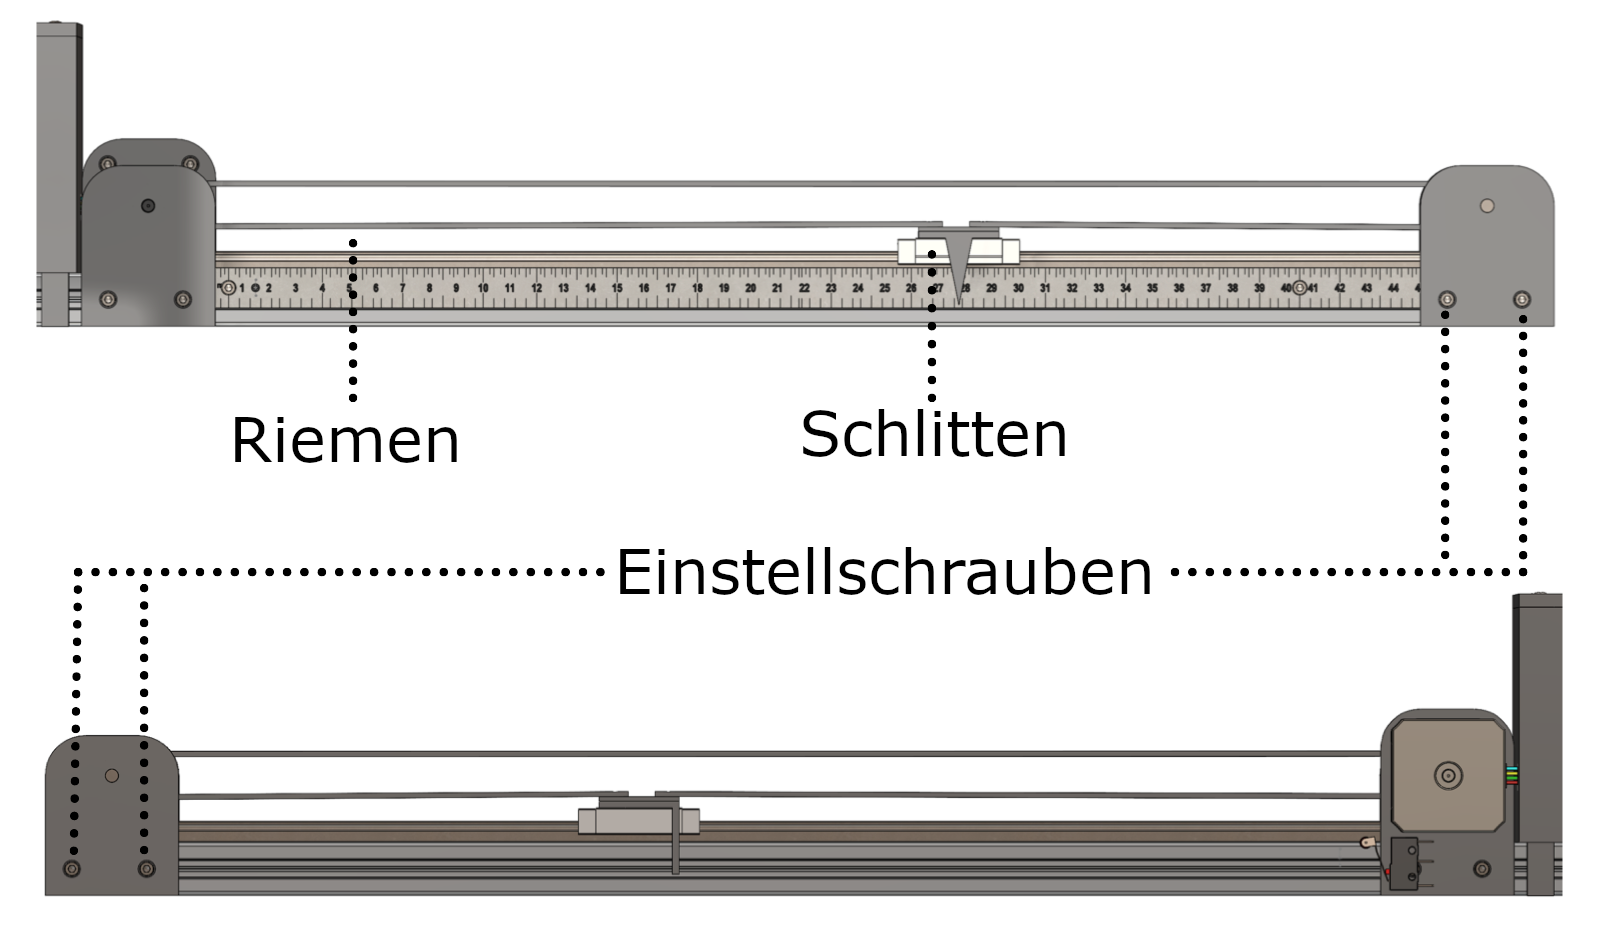
\includegraphics[width=\textwidth]{Images/Konstruktion4.png}
	%	\caption{Dies ist eine Konzeptskizze und wird noch ausgetauscht} \label{-}
	%	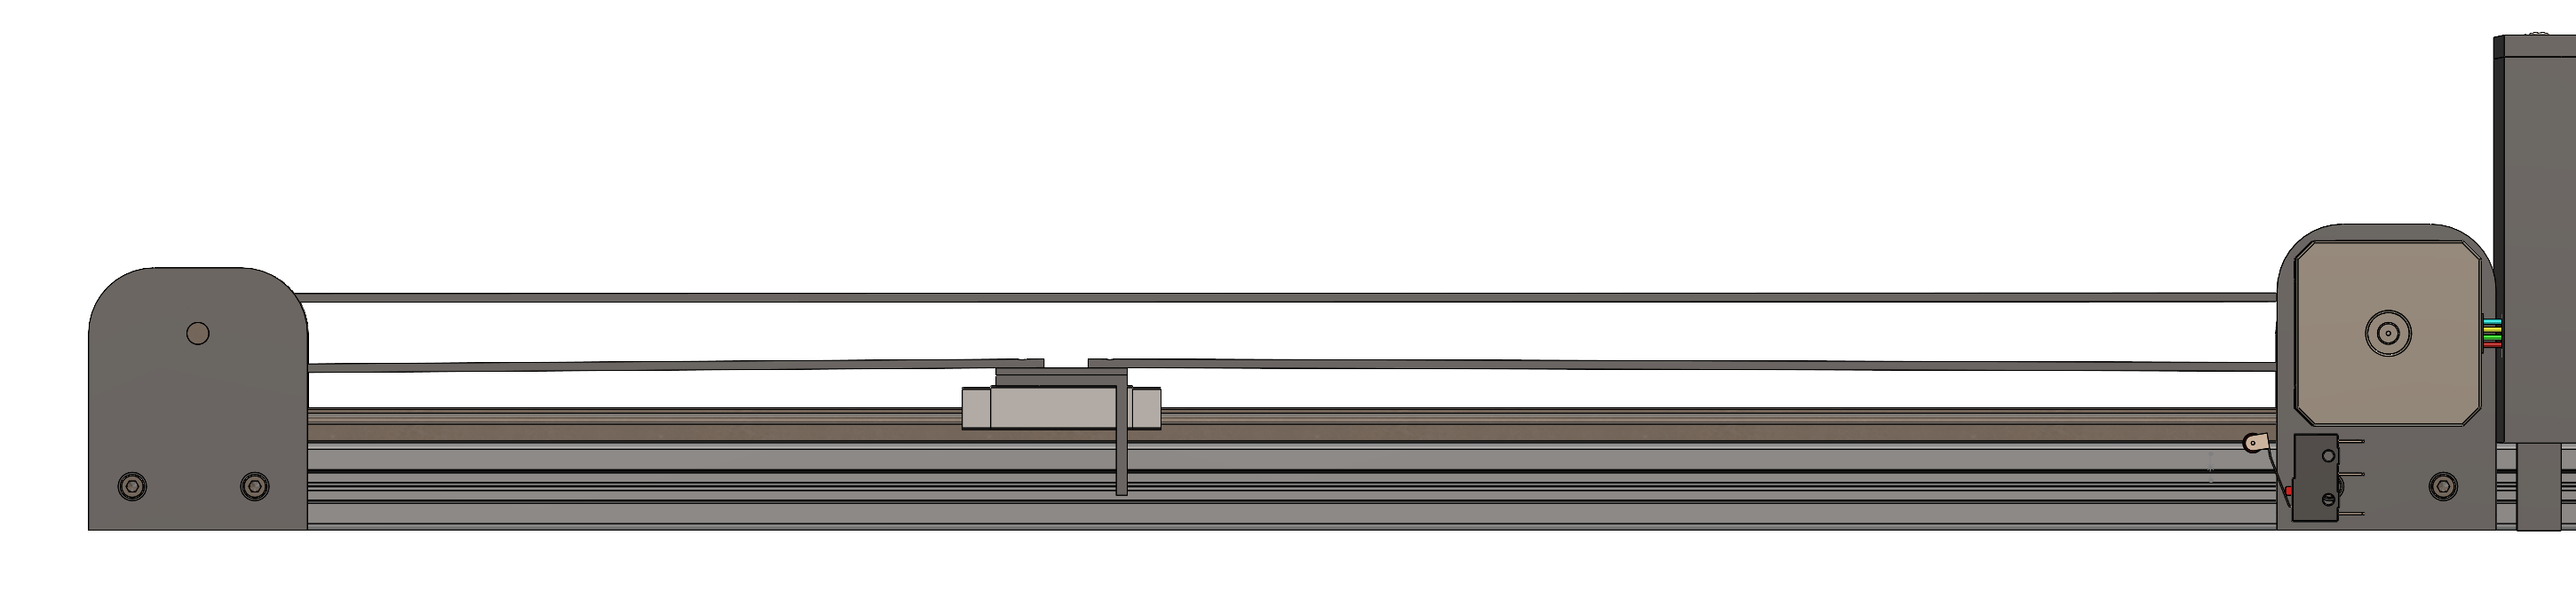
\includegraphics[width=\textwidth]{Images/Konstruktion5.png}
	%	\caption{Dies ist eine Konzeptskizze und wird noch ausgetauscht} \label{-}
\end{center}
	\textbf{Riemen}
\begin{itemize}
	\item Notwendiges Bauteil zum verfahren des \textbf{Schlittens} .
\end{itemize}
\textbf{Einstellschrauben}: 
\begin{itemize}
	\item Notwendig zum Spannen des Riemens siehe \glqq Elastische Einstellung des Riemens \grqq auf \ref{STU} \nameref{STU}. 
\end{itemize}
\textbf{Schlitten}: 
\begin{itemize}
	\item Verfahrelement  
\end{itemize}



